\documentclass[11pt]{article} % use larger type; default would be 10pt

% Common packages for mathematical articles
\usepackage{fullpage,amsmath,amsfonts,mathpazo,microtype,nicefrac,algorithm2e,graphicx}

% MSE Packages
\usepackage{caption}
\usepackage{physics}
\usepackage{xcolor}
\usepackage{listings}
\usepackage{parskip}

% MSE Make margins a bit smaller
\usepackage[margin=0.75in]{geometry}
\usepackage[font=footnotesize]{caption}

% MSE set graphics path
\graphicspath{{../figs/}}

% Set-up for hypertext references
\usepackage{hyperref,color,textcomp}
\definecolor{webgreen}{rgb}{0,.35,0}
\definecolor{webbrown}{rgb}{.6,0,0}
\definecolor{RoyalBlue}{rgb}{0,0,0.9}
\hypersetup{
   colorlinks=true, linktocpage=true, pdfstartpage=3, pdfstartview=FitV,
   breaklinks=true, pdfpagemode=UseNone, pageanchor=true, pdfpagemode=UseOutlines,
   plainpages=false, bookmarksnumbered, bookmarksopen=true, bookmarksopenlevel=1,
   hypertexnames=true, pdfhighlight=/O,
   urlcolor=webbrown, linkcolor=RoyalBlue, citecolor=webgreen,
   pdfsubject={Harvard IACS AC 290 R},
   pdfkeywords={},
   pdfcreator={pdfLaTeX},
   pdfproducer={LaTeX with hyperref}
}
\hypersetup{pdftitle={AC290-RBC}}


% MSE Macros
\newcommand{\tty}[1]{\texttt{#1}}
\newcommand{\uu}{\vectorbold{u}}
\newcommand{\vv}{\vectorbold{u}}
\newcommand{\Laplace}{\Delta}
\renewcommand{\vec}[1]{\mathbf{#1}}

%***Start of Document***
\title{Hemodynamic Simulation with Lattice Boltzman}
\author{Harvard IACS AC 290R - Group 1 \\
Michael S. Emanuel \\
Jonathan Guillotte-Blouin \\
Yue Sun \\
}
\date{28-April-2019} 

\begin{document}
\maketitle

\section{Problem Statement and Motivation}
AC 290R is a course on extreme computing with a focus on the application domain of fluid dynamics.
In our first module we attempted a prototypical problem using the continuum description of fluids
governed by the Navier-Stokes equation: 
\href{https://en.wikipedia.org/wiki/Rayleigh%E2%80%93B%C3%A9nard_convection}{Rayleigh-B\'enard Convection}.
In this module, we shift from the continuum to the mesoscale description and simulate fluids using  
\href{https://en.wikipedia.org/wiki/Lattice_Boltzmann_methods}{Lattice Boltzmann} methods.  
These methods are based on the Boltzmann Equation of thermodynamics and statistical physics.

The particular task we we undertook was a hemodynamic simulation.
\href{https://en.wikipedia.org/wiki/Hemodynamics}{Hemodynamics} is the study of the dynamics flow blood.  
It is a rich field at the intersection of anatomy and physics with a storied history.
Pioneers in the field have included 
\href{https://en.wikipedia.org/wiki/Leonardo_da_Vinci}{Leonardo Da Vinci}, 
\href{https://en.wikipedia.org/wiki/Leonhard_Euler}{Leonhard Euler,} 
\href{https://en.wikipedia.org/wiki/Thomas_Young_(scientist)}{Thomas Young}, and 
\href{https://en.wikipedia.org/wiki/Jean_L%C3%A9onard_Marie_Poiseuille}{Jean L.M. Poieseuille}.

The particular problem was as follows.  
We aim to model the dispersion of a therapeutic drug that is injected with a catheter to treat a stenotic artery.
Stenosis is a disease of the arteries in which an artery becomes narrowed.
It is frequently caused by 
\href{https://en.wikipedia.org/wiki/Atherosclerosis}{atherosclerosis}, 
a build-up of fatty deposits (cholesterol) on the walls of the artery.
Stenotic arteries can cause serious medical problems including heart attacks and strokes.
One approach to treating stenoses is to introduce a therapeutic drug with a catheter,
a small tube inserted surgically into the patient that can be threaded through the circular system.
The goal of our simulation was to understand how the drug molecules dispersed 
and to see how many of them passed through the stenotic region, and at what times.

This is a worthwhile object of study for both pedagogical and practical reasons.
Pedagogically, this topic rounds out our survey of both techniques and domain knowledge in the course.
We are aiming to master the techniques of extreme computing and their application to fluid dynamics.
The first topic covered the continuum approach, and this topic covers the mesoscale approach.
The first topic used traditional CPU-centric computations, and this topic introduces us to GPU computing.

On a practical level, \href{https://www.cdc.gov/heartdisease/facts.htm}{heart disease} 
has been for many years a leading cause of death in Americans alongside cancer.
It is a complex disease with many treatment options and a need for accurate diagnosis.
Clinical practice still often relies on human judgment about which arterial blockages 
look risky, and there is reason for optimism that advances in biologically realistic computer
simulations could lead to materially faster and more accurate diagnosis 
and improve treatement selections.

\newpage
\section{Overview of Numerical Methods Used}
The main numerical method used in this simulation is the Lattice Boltzmann Method (LBM).
LBM is based on the \href{https://en.wikipedia.org/wiki/Boltzmann_equation}{Boltzmann Equation},
which describes the statistical behavior of a thermodynamic system and dates to 1872.
The idea behind the Boltzmann Equation is that particles in the system each have 6 degrees
of freedom, 3 positions and 3 momenta along the 3 coordinate directions $x$, $y$ and $z$.
Molecules of a given type are physically indistuinguishable from each other,
so the system can be described completely by the populations of particles as a function
of time and these six dimensions in the phase space.
The Boltzmann Equation describes the evolution of such a system.
The populations of particles change due to three terms: 
forces applied to the system, diffusion, and collisions.

LBM is a technique in computational fluid dynamics that uses the Boltzmann Equation
to devise a numerical simulation of a fluid that can accurately capture mesoscale dynamics
when it is tuned properly.
The physical system is discretized, typically on a rectilinear grid 
and most commonly one with cubic spacing.  
Particle velocities are also discretized, with particles allowed to jump from
from one grid point only to nearby grid points over one simulation step.
The most common discretization scheme for 3D fluid simulations,
which we used for this problem, is called D3Q19.
The label can be parsed as referring to 3 dimensions and 19 discrete velocities.
The 19 discrete velocities have the following structure:
\begin{itemize}
\item 1 $0^{th}$ neighbor; displacement $(0,0,0)$; weight $\frac{1}{3}$
\item 6 $1^{st}$ neighbors; displacement one of 3 permutations of $(\pm 1, 0, 0)$; weight $\frac{1}{18}$
\item 12 $2^{nd}$ neighbors; displacement one of 3 permutations of $\pm 1, \pm 1, 0)$; weight $\frac{1}{36}$
\end{itemize}
The 6 first neighbors have displacements $(1,0,0), (-1,0,0), (0,1,0), (0,-1,0), (0,0,1), (0,0,-1)$.
The 12 second neighbors follow a similar pattern; there are ${3 \choose 2} = 3$ permutations of indices
$i, j$, and each index has 2 choices in $\pm1$, leaving $4 \cdot 3 = 12$ second neighbors.
The total weight of the 6 first neighbors is $6 \cdot \frac{1}{18} = \frac{1}{3}$.
The total weight of the 12 second neighbors is $12 \cdot \frac{1}{36} = \frac{1}{3}$.

The state of the simulation at a time step is given the \textit{population} of particles, 
$f_p(x,t)$, where the suffix $p$ refers to the discrete velocities above.
In a system with more than one type of particle, each populations of each particle must be maintained separately.  
The movement of populations can be described by the Btatnagar-Gross-Krook update rule:
$$f_p(x + hc_p, t + h) = f_p(x,t) + \omega(x,t) h \left[f_p^{eq}(\rho, \vec{u} - f_p)(x,t) + w_p \frac{c_p \cdot \vec{g}}{c_s^2} \right]$$
Here is a brief description of all the terms appearing in this equation from left to right:
\begin{itemize}
\item $f_p$ is the actual population of the particle introduced above.
\item h is the time step, often taken to be 1 in simplified notation
\item $c_p$ is the displacement vector corresponding a given discrete velocity, e.g. \\
$c_0 = (0,0,0)$,  $c_1 = (1,0,0)$, etc.
\item $\omega$ is the relaxation frequency which is related to the kinematic viscosity $\nu$ (described below)
\item $\rho(x,t)$ is the density of the fluid in this cell, a macroscopic quantity; essentially the 0th moment of the velocity
\item $\vec{u}(x,t)$ is the velocity of the fluid in this cell, a macroscopic quantity; essentially the first moment of the velocity
\item $w_p$ is the weight of particles with each velocity in the D3Q19 scheme; scalars that do not change over the simulation
\item $c_p$ is the discrete velocity
\item $\vec{g}$ is the acceleration applied to the body by external forces; the letter $g$ evokes gravity but it can be any external force
\item $c_s$ is the speed of sound in dimensionless units on this lattice. 
(The speed of sound of the physical medium depends on the gradient of pressure with respect to density).
\end{itemize}

The equilibrium populations can be approximated with a Taylor expansion that
accounts for the 0th, 1st, and 2nd moments of the populations.
$$f_p^{eq}(\rho, \vec{u}) = w_p \rho \left[1 + \frac{\vec{u} \cdot c_p}{c_2^2} + \frac{(\vec{u} \cdot c_p)^2 - c_s^2u^2}{2c_2^4} \right] $$
The resulting $f_p^{eq}$ will match the first two moments (density $\rho$ and velocity $\vec{u}$),
but in general it will $\textbf{not}$ match the second moment (energy density) unelss the system is at equilibrium.
This is how energy dissipation in a viscous fluid away from equilibrium is modeled.
This approximation is valid as long as the system is sufficiently close to equilibrium.
If the parameters are not set properly, the populations can depart from equilibrium by too much
and the simulation will break down.

The macroscopic quantity density $\rho$ is simply the sum of the fluid populations in a cell.
$$\rho(\vec{x}, t) = \sum_{p}f_p(\vec{x}, t)$$
The momentum density is the first moment of the particle velocities.  
This is equal to the density times the velocity in a cell, giving us the formula for $\vec{u}(\vec{x}, t)$:
\begin{align*}
\vec{J}(\vec{x}, t) &= \rho(\vec{x}, t) \vec{u}(\vec{x}, t) = \sum_{p}c_p f_p(\vec{x}, t) \\
\vec{u}(\vec{x}, t) &= \frac{1}{\rho(\vec{x}, t)} \sum_{p}c_p f_p(\vec{x}, t)
\end{align*}

The relaxation frequency is related to the kinematic viscosity $\nu$ by the following relationship:
$$ \nu = c_s^2 \left(\frac{1}{\omega} - \frac{1}{2}\right)$$

A Lattice Boltzmann fluid simulation can be organized into two logical phases, 
which are sometimes called \textit{collision} and \textit{streaming}.
The collision step describes how particles populations in the same cell interact and 
how their weights move toward their equilibrium values as a result of collisions.
The intuition is that when particles hit each other, momentum is conserved, 
but some kinetic energy is dissipated as heat or otherwise.
The equation for the collision step can be written
$$f_p^* = (1-\omega)f_p + \omega f_p^{eq}$$
where $f_p^*$ are called the temporary post-collisional populations.
We can think of these as the new populations one ``instant'' after the previous streaming step.

The streaming step describes how particles of the post-collisional population move forward into the next time step.  
This is very straightforward, the particles just move at their discrete velocities according to
$$f_p(x + c_p, t+ 1) = f_p^*(x, t)$$
A key fact is that streaming is a \textit{local} operation.  
This makes it ideally suited to GPU computations, which excel at simple, highly parallel tasks with memory locality.

Stability is an important concept in the numerical solution of differential equations generally.
One of the best known stability criteria is the 
\href{https://en.wikipedia.org/wiki/Courant%E2%80%93Friedrichs%E2%80%93Lewy_condition}{Courant-Friedrichs-Lewy (CFL) Condition}.
This relates the range of time steps $\Delta t$ for which a numerical method is stable to the spatial discretication $\delta x$,
the speed of movement $u$, and a dimensionless constant that is a property of the numerical method.
A rule of thumb for LBM is that optimal results are achieved when 
$$|u| < \sqrt{\frac{2}{3}} \frac{\Delta x}{\Delta t}$$
A representative value of $u$ is 0.1, leading to a guideline that stable results can be found when the
kinematic viscosity $\nu$ is selected in the range $0.05 < \nu < 1$.

Like any differential equation solution method, LBM must also cope with initial conditions and boundary conditions.
Common initial conditions are prescribed values for the pressure (equivalent to a prescribed density)
and velocity, i.e.
\begin{align*}
\rho(x, t=0) &= \rho_0(x) \\
\vec{u}(x, t=0) &= \vec{u}_0(x)
\end{align*}
A common choice is to set the initial density to be uniform and the initial velocity to be zero.
Once $\rho$ and $\vec{u}$ are initialized, a common modeling choice is to initialize the
populations to the equilibrium implied by these macroscopic variables, i.e.
$$f_p(x, 0) = f_p^{eq}(\rho_0(x), \vec{u}_0(x))$$

Boundary conditions are a bit trickier.  
An astute reader will quickly point out that with these equations as written,
any finite domain will have particles ``falling off the edge'' and without
sensible treatment of boundary conditions, the simulation would just report
that there were no particles left.  That would be sad.
In general, a boundary condition in an LBM simulation can be expressed as 
a linear combination of a constraint on the flux in a direction normal to a wall,
and on the density itself.  
Taking $\phi$ to denote the quantity of interest (can be density or velocity) 
and $n$ the normal direction,
$$b_1 \frac{\partial \phi}{\partial n}(x_b, t) + b_2 \phi(x_b, t) = b_3$$ 

A few special cases are the most common.  
When $\phi = \vec{u} = 0$, we have the \textbf{no slip} boundary condition.
This is common and physically realistic.
When $b1 = 0$, we have a Dirichlet boundary condition, in which the value is imposed.
When $b2 = 0$, we have a Neumann boundary condition, in which the flux is imposed.
When $b1 \ne 0$ and $\b2 \ne 0$, the boundary condition is mixed 
(linear relationship between field value and flux) and is called a Robin boundary condition.
In addition to no-slip boundary conditions, another common choice is for velocity
to be fixed at an \textit{inlet} or \textit{outlet}.
Finally, larger sytems can often be simulated using a \textit{periodic} boundary condition.
For the simulation we ran of an artery, we imposed a non-slip boundary condition on the
side walls of the artery, and a periodic boundary condition on the longitudinal direction,
effectively modeling a longer artery with periodic stenoses.

\newpage
\section{Description of Code}
The workhorse of this simulation is a Lattice Boltzmann fliud simulator called MUPHY.
MUPHY is about 10 years and designed for multi-physics simulations.
We also used a newer software package called MOEBIUS.
MUPHY is an open source project on which our guest instructor Simone Melchionna
was one of the lead developers
MOEBIUS is a commercial package developed by a private company,
Lexma, founded by Dr. Melchionna.

MUPHY and MOEBIUS (hereafter referred to simply as MUPHY to save space) follow a similar strategy to Drekar.  
They are object oriented written primarily in a mix of C / C++ and Fortran, with GPU acceleration written in Cuda.
The back end is implemented in lower level languages like C / C++  to meet the requirements for high performance.
Another similarity to Drekar is that parallelization is proved using OpenMP.
There is also a front end interface for managing jobs.  This is written in Python.
To run our simulations, we needed to install the MUPHY package and write
scripts in Python.  We did not need to write or compile and C++ or Cuda.

MUPHY was written with a particular focus on applications in life sciences.
It can handle the complex geometries arising in biological systems, ranging in scales
from folding proteins and cell membranes up to highly branched arteries.
We saw demonstrations in class run on MUPHY of a DNA molecule passing through
a cell membrane, and of a flow simulation in arteries whose geometry was
based on a patient.

The first code we wrote is in the file \tty{ShapePainter.py}.
This code can be found in a repository named BUFFY our team created on Odyssey.
We needed to fork the MUPHY repository so we could make edits and push changes.
We named it BUFFY in homage to the hit TV show 
\href{https://en.wikipedia.org/wiki/Buffy_the_Vampire_Slayer}{Buffy the Vampire Slayer}.
Access to this repository can be provided to the teaching staff on request.
We took snapshot of the most relevant Python scripts and saved them in our
team repository (where we submit our coursework) in the directory \tty{/project2/BUFFY}.
\tty{ShapePainter.py} creates a geometry for the system using the \tty{vtk} library.
The artery is modeled with a simplified geometry 
as a cylinder extending down the $z$ axis longitudinally.
It has a radius $R$ on the healthy region and $G=R/2$ in the stenotic region.
The length of the entire artery is $L$ and the length of the stenotic region is $S$.
This image was provided with the problem statement and demonstrates
the basic layout and parameter names:
\begin{figure}[h!]
\centering
%\hspace*{-0.25in}
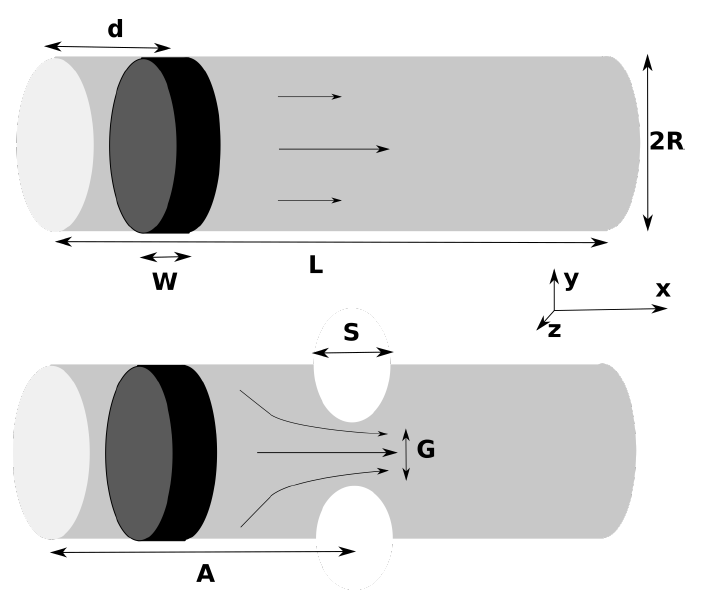
\includegraphics[width=0.40\textwidth]{artery_geometry.png}
\caption{Artery Geometry.}
\end{figure}

\colorbox{yellow}{IMAGE OF ACTUAL GEOMETRY WE GENERATED}

\colorbox{yellow}{YUE TO SAY MORE ABOUT SHAPE PAINTING SCRIPT AND RUNS}

The next code we wrote is the Python script that runs the simulation on MUPHY.
Each simulation run had a file, conventionally named \tty{run2.py}, that kicks off the simulation.  
The script that ran our baseline simulation is located in 
\tty{scratchlfs/ac290r/project2/blood\_cells/BUFFY/RBC\_0\_Re10}
(We tried to follow advice given to use organized directory names.
While this is a bit long and slightly cryptic, we did at least follow a consistent scheme
this time organized everything hierarchically!)
We've included a copy of this file in project repository as well in
\tty{project2/BUFFY/RBC\_0\_Re10} for convenience in grading our submission.

The first part of this file sets the physical parameters for the simulation,
e.g. the geometry of the cylinder and the viscosity.
The Python module \tty{MagicUniverse} is the fancifully named interface to the BUFFY simulation engine.
The script initializes simulation objects including:
\begin{itemize}
\item Universe
\item Scale
\item Mesh
\item Fluid (for blood)
\item Fluid (for drug)
\item Tracker (for diagnostics)
\end{itemize}
These are all class instances from the \tty{MagicUniverse} module.
Parameter values are set to the appropriate class instances.
We set the boundary conditions to be periodic on the $z$ axis,
and no-slip on the $x$ and $y$ axes.
The alternative configuration would have been to create inlets and outlets
at the start and end values of $z$.

\colorbox{yellow}{YUE TO SAY MORE IF NECESSARY}

To run this code on Odyssey (Harvard's supercomputing cluster in Western Massachusetts)
we also wrote shell scripts that were submitted to the Odyssey job manager \tty{slurm}.
The script to run the baseline simulation is called \tty{runrbc\_0.sh} and is located adjacent to \tty{run2.py}.  
The key lines in this script set the job options and load the required modules.  
Important flags include:
\begin{itemize}
\item \tty{-p shared} - run the job on the shared partition
\item \tty{--reservation=ac290r} use the reservation so we don't have to wait in the queue to get 1024 CPUs 
\item \tty{-t 1200} hold the job open for up 1200 minutes = 20 hours
\item \tty{-n 512} run on a total of 512 CPU cores
\item \tty{N 16} run on 16 nodes; we are therefore requesting 16 nodes with 32 cores each
\item \tty{mem=64000} request 64,000 MB = 64 GB per node; that is a lot of memory, 1024 GB = 1 TB total
\item \tty{--job-name=RBC0RE10} the descriptive job name refers to 0 red blood cells and Reynolds Number 10
\item \tty{--output=RBC0RE10.out} the directory where output is written; matches the job name
\end{itemize}

The rest of the script loads the required modules and sets environment variables.
We need modules for \tty{gcc} and \tty{openmpi}, provided by 
\tty{gcc/7.1.0-fasrc01} and \tty{openmpi/3.1.1-fasrc01} respectively.
The environment variables to set are \tty{MOEBIUS\_PATH} and \tty{PYTHONPATH}.
These allow Python to find the MAGIC modules.
In order to invoke the job as a Python 2 script with MPI, the 
line of the script that kicks off the actual job is\\
\tty{srun -n \$SLURM\_NTASKS --mpi=pmi2 python2 run2.py}

The last major batch of code we wrote performs calculations at the post-processing stage.
This is in two Python scripts \tty{vtk2np.py} and \tty{rbc.py} located in the folder \tty{project2/src}.
The MUPHY simulation generates output in the form of VTK files with the extensions .vtu and .pvtu.
These files are well suited to visualization, especially intensive visualizations like movies.
For computations and 2D plots of one time instant, we find it more convenient to use 
\tty{numpy} and \tty{matplotlib}.

We made a strategic decision to do the computationally heavy graphics rendering remotely on Odyssey
but to do the computations and 2D ploting locally on a few selected time frames.
After our baseline simulation ran, we downloaded snapshots every 100,000 frames from 100,000 to 1,000,000.
Each time step corresponds to 1 microsecond, so these frames were 100 milliseconds apart for
the first 1.0 second of the simulation.  
These files weren't too large, with a total size of about 9 GB each for the blood and drug for a total of 18 GB.
Downloading these files was a bit painful though because SFTP connections to Odyssey 
are considerably slower than data downloads from large commercial websites for whatever reason.

The script \tty{vtk2np.py} converts the VTK files to numpy arrays using the library \tty{vtki}.
\tty{vtki} has a nice feature making it possible to read a .pvtu file.  
A .pvtu file is essentially a wrapper around a number of .vtu files, each with one part of a larger mesh.  
In our case, we ran on 512 nodes and each time step generated 512 .vtu files that were summarized by 1 .pvtu file.  
These outputs were generated for both blood and the drug.
The VTK files include data that is keyed both by \textit{points} and \textit{cells} on the mesh.
These are not the same! Our mesh for $Re=10$ had 7,022,647 cells and 8,578,503 points.
One important optimization is to realize that the geometric layout of the mesh does not change between frames.  
While the files contain the whole grid every time, it is only necessary to save the point and cell position data once.  
Only the density, velocity, and shear stress change over frames.

\tty{vtk2np.py} extracts and saves the following data from the VTK files as Numpy arrays:
\begin{itemize}
\item \tty{point\_pos.npy} - the (x, y, z) position of each point on the mesh
\item \tty{cell\_pos.npy} - the (x, y, z) position of each cell center of the mesh
\item \tty{cell\_vol.npy} - the volume of each cell in the mesh
\item \tty{drug\_framenum.npy} - the volume of the drug in each cell of the mesh at this frame
\item \tty{drug\_point\_framenum.npy} - the volume of the drug at each point on the mesh at this frame
\item \tty{vel\_framenum.npy} - the blood velocity at each point on the mesh at this frame
\item \tty{vel\_cell\_framenum.npy} - the blood velocity at each cell on the mesh at this frame
\item \tty{rho\_framenum.npy} - the blood density at each cell on the mesh; proportional to pressure
\end{itemize}
This program was run once locally to create numpy arrays, allowing the
next Python program to run without worrking about VTK data structures.

\tty{rbc.py} performs all the requested calculations and generates the 2D plots presented 
below that were not generated remotely using Paraview. \\
\tty{drug\_delivery} answers the headline question of how much drug is in the stenotic
region as a function of time.  
We estimated this by summing up the density of drug in the cells in the stenotic region.
We extracted the velocity of each cell and found that they were all equal to 1.
(We knew that the interior cells should have a volume of 1 because they were cubes
with side length 1, but didn't know how MUPHY and VTK handle cubes on the boundary.)
The total amount of drug present in a region $\Omega$ is $\int_{\Omega} \rho dV$
i.e. the density integrated with respect to infinitesimal volume slices.
Therefore discrete analog would be to sum up the density of each cell in the stenotic region multiplied by its volume.  
Since all the cell volumes are equal to 1, we omitted the multiplication from the calculation to improve performance.
We also computed the total quantity of drug in the system as a quality check, expecting it not to change.\\
\tty{plot\_speed\_contour} creates a contour plot of the speed on a cross sectional slize $z=z_{plot}$.
While we computed drug quantities using cells, we chose to plot speed using points.
The main programming challenge is generating a contour for data that doesn't cover an entire rectangular grid.
This was done by creating an augmented grid with the full square cross section containing
the circular cross section of the artery.
Grid points outside of the artery were marked with a speed of 0, which was exlcuded from the
range of values in the contour.\\
\tty{plot\_streamlines} plots streamlines of the velocity in the $xy$ plane
(i.e. velocity components $u$ and $v$) on a cross-sectional slice $z=z_{plot}$.
Like the speed contour, this plot uses points rather than cells.
It uses the same technique as \tty{plot\_speed} for padding the circular region
with dummy entries that don't appear on the plot.
Streamlines are plotted with a width proportional to their speed in the $xy$ plane.\\
\tty{plot\_drug\_conc} plots the concentration of the drug on a cross sectional slice $z=z_plot$.
This plot uses cell data.  
A mask is created using the relationship that $z$ at the center of a cell is equal to 
$z$ at the start of the cell plus $\frac{1}{2}$.  
This was preserved exactly by VTK so we could create a logical mask efficiently.
The conentration of drug at each $(x, y)$ point is then read right off the masked array.\\
\tty{plot\_drug\_profile} plots the ``profile'' of the drug along the $z$ axis for a given time.
This calculation is also based on cells.  
A mask is created for each value of $z$ as before, and the total amount of drug 
at this longitude is estimated as the sum of the drug concentration array on the mask.
An initial attempt at plotting this profile showed some obvious artifacts where 
a handful of $z$ values had ``holes'' where the dropped well below their neighbors.
We appplied a smoothing operation before plotting the profile $B(z)$ in which 
we set each $b_z$ equal to the max of itself and its two neighbors $b_{z-1}$ and $b_{z+1}$.\\
Plots of each type are displayed below in the Results section.

\section{Parameters of the Simulation}
These are the parameter values that we set at the start of the Python script for the baseline simulation
with 0 red blood cells and a Reynold Number of 10.
\begin{itemize}
\item $\nu$ = 0.1 - this is the kinematic viscosity
\item $\rho$ = 1 - the blood density wsa set to 1 by convention
\item $\bar{u}$ = 0.01 - this is the mean speed of the blood
\item Re = 10.0 - the Reynolds number is dimensionless and characterize the turbulence / regularity of the flow
\item Pe = 10.0 - the Pectet number is dimensionless and characterizes the importance of radial to axial diffusion
\item R = $\nicefrac{Re * \nu}{2  \bar{u}}$ - the radius is implied by Reynolds number and velocity
\item DIFFUSIVITY = $\frac{\bar{u} * R}{Pe}$ \colorbox{yellow}{SAY SOMETHING HERE}
\item C0 = 0.01 - the baseline drug concentration away from the bolus
\item C1 = 1.0 - the high drug concentration on the bolus at $t=0$
\item NSTEP = 1000000 - total number of simulation steps; each step is one microsecond
\item NDIAG = 100 - interval between diagnostics
\item NVTKFREQ = 1000 - interval between VTK output frames
\item UNFREEZE\_TIME = 100000 - number of time stepss for the system to equilibrate before drug release
\end{itemize}

Our goal was to also run a big simulation.  
This was to be similar to the baseline, but would also include a large number of red blood cells.
These red blood cells would be simulated as rigid particles with a position and orientation.
Including the red blood cells makes the simulation more physiologically realistic,
with increasing importance the narrower a blood vessel is.
Our initial attempt was a 30\% hematocrit with otherwise identical parameters to the baseline case.  
Unfortunately multiple attempts to simulate the system with large numbers of red blood cells failed.
We will explain in detail the various failures and their causes in the section below.
Fortunately, we did complete a successful run of the baseline case without red blood cells.
We have made the best of a difficult situation by perofrming a complete analysis on the baseline case.

\section{Results}

\subsection{Failed Runs on Odyssey with Red Blood Cells}

\subsection{Drug Delivery Over Time}

\subsection{Velocity Field - Contours of Speed and Streamlines}

\subsection{Drug Concentration - Contours}

\subsection{Longitudinal Drug Profile vs. Time}

\section{Conclusions and Future Work}

%% bibliography

\begin{thebibliography}{9}
\bibitem{exo} 
Succi, Sauro: The Lattice Boltmann Equation for Fluid Dynamics and Beyond

\end{thebibliography}

\end{document}

